\chapter{Reimplementation of MoSeL in Ltac2}
\label{chap:reimplementation_ipm}

The original implementation of Iris Proof Mode is due to \citet{krebbersInteractiveProofsHigherorder2017}.
It was later extended to MoSeL by \citet{krebbersMoSeLGeneralExtensible2018}, a general framework for modal separation logics in Coq.
However, while the original work was done using Ltac1, here we present a translation of MoSeL to Ltac2.
In the translation we follow both its ideas and implementation closely.

The structure of the chapter is as follows:
\begin{itemize}
\item First we describe the basics of separation logic and basic semantics.
\item Then we cover the embedding of logic in Coq and how MoSeL entailments correspond to the theory.
\item Afterwards we go into the details of the implementation of tactics and proof mode.
\item Finally, we share some experiences from the translation of Ltac1 implementation to Ltac2.
\end{itemize}

\section{Introduction to separation logic}
\label{sec:separation-logic-intro}

We will now describe the basics of the separation logic.
Separation logic is an extension of Hoare logic which includes several new operators, the most important two being separating conjunction \((*)\) and separating implication or ``magic wand'' \((\wand)\).
Separation logic is also built on Bunched Implications logic.

A BI logic is a set of propositions \Prop with an entailment predicate \(\vdash\) and the following connectives:
\begin{enumerate}
\item embedding of ``pure'' propositions from meta-logic, which don't concern resources: \(\pure { } : \textbf{Prop} \to \Prop\)
\item \True, a neutral element for non-separating conjunction \(\wedge : \Prop \to \Prop \to \Prop\)
\item \False, a neutral element for non-separating disjunction \(\vee : \Prop \to \Prop \to \Prop\)
\item \emp, a neutral element for separating conjunction \(* : \Prop \to \Prop \to \Prop\)
\item \(\imp\) and \(\wand\), two implication-like connectives, where only the latter is separating.
\item quantifiers, since the logic is higher-order: \(\forall, \exists : \forall A, (A \to \Prop) \to \Prop\)
\end{enumerate}

Apart from the laws concerning neutral elements mentioned above, there are laws concerning introduction and elimination of connectives, as well as the usual properties like commutativity and associativity.

The connectives that differentiate BI logic from regular one are separating conjunction (\(*\)) and magic wand (\(\wand\)).
Intuition behind BI logic is somewhat simpler to understand by example.
In classical separation logic \cite{reynoldsSeparationLogicLogic2002, ohearnLocalReasoningPrograms2001}, a prototypical instance of a BI logic, propositions predicates on memory heaps.
In that case a separating conjunction \(P \ast Q\) means that the heap can be divided in two heaplets, such that they don't share any memory and each one satisfies one the propositions respectively.
Separating implication \(P \wand Q\) means that any heaplet that satisfies \(P\) also satisfies \(Q\).
Lastly, the neutral element \emp simply means that a heaplet is empty.
Non-separating conjunction \(P \wedge Q \)in that case means that the heaplet satisfies both \(P\) and \(Q\) simultaneously.

Entailment predicate for BI takes a ``bunch'' for the context and a proposition for the goal.
Bunches can be formed by two connectives -- ``additive'', which is represented as a semincolon, and ``multiplicative'', which is represented by a comma.
The bunches are introduced by the following two introduction rules:
\begin{equation*}
  \infer[\imp R]
        {\Gamma \vdash P \imp Q}
        {\Gamma ; P \vdash Q}
  \quad \quad
  \infer[\wand R]
        {\Gamma \vdash P \wand Q}
        {\Gamma , P \vdash Q}
\end{equation*}
Intuitively, additive bunch corresponds to the non-separating conjunction, while the multiplicative bunch -- to the separating one, respectively.
\begin{equation*}
  \infer{P \wedge Q \vdash R}
        {P ; Q \vdash R}
  \quad \quad
  \infer{P \ast Q \vdash R}
        {P, Q \vdash R}
\end{equation*}
The important distinction, however, is that additive bunches admit the rules of Weakening and Contraction, while in classical BI multiplicative bunches do not.
This is also reflected by the introduction rules for conjunctions:
\begin{equation*}
  \infer[\wedge R]
        {\Gamma \vdash P \wedge Q}
        {\Gamma \vdash P &
         \Gamma \vdash Q }
  \quad \quad
  \infer[\ast R]
        {\Gamma, \Delta \vdash P \ast Q}
        {\Gamma \vdash P &
         \Delta \vdash Q }
\end{equation*}

For more careful treatment of BI logic the user is referred to the original works \cite{ohearnLogicBunchedImplications1999, pymSemanticsProofTheory2002a}.
We are, however, more interested in the separation logic, which uses BI logic to describe programs.

\paragraph{Classical separation logic.}
We mentioned it as an intuitive explanation behind BI logic and we describe it slightly more detailed.
In classical separation logic \cite{ohearnLocalReasoningPrograms2001, reynoldsSeparationLogicLogic2002}, propositions are predicates over memory heaps, so we take memory to be a map from locations to values: \(\sigma \in \textit{State} \delequal \mathbb{N} \xrightarrow[]{\text{fin}} Val\) and then propositions are modeled as \(P \in \Prop \delequal \textit{State} \imp \textbf{Prop}\).

The connectives are then defined in such a way to preserve these semantics:
\begin{itemize}
\item \(\emp \delequal \lambda \sigma. \sigma = \emptyset\)
\item \(\l \mapsto v \delequal \lambda \sigma. \sigma = [l \leftarrow v]\)
\item \(P \wedge Q \delequal \lambda \sigma. P (\sigma) \wedge Q (\sigma)\)
\item \(P \ast Q \delequal \exists \sigma_1, \sigma_2. \sigma = \sigma_1 \uplus \sigma_2 \wedge P(\sigma_1) \wedge Q(\sigma_2)\)
\end{itemize}

\paragraph{Intuitionistic separation logic.}
Another canonical instance of BI logic is intuitionistic separation logic \cite{reynoldsIntuitionisticReasoningShared2000}.
Unlike in classical SL, here propositions are modeled by predicates, which are monotone with respect to inclusion order \(\subseteq\) on heaps and implications in \textbf{Prop}.
To reflect this, definitions of connectives has to be changed:
\begin{itemize}
\item \(\emp \delequal \lambda \sigma. \True \)
\item \(\l \mapsto v \delequal \lambda \sigma. [l \leftarrow v] \subseteq \sigma \)
\end{itemize}

Intuitionistic logics are better suited for reasoning about programs with garbage collection, since, due to monotonicity, they allow us to ``forget'' about some parts of the memory: \(l \mapsto v \ast P \vdash P\), for any \(P\).

\paragraph{Affine logics.}
This ability to ``forget'' can also be expressed in the BI logics directly.
There, it corresponds to the presence of weakening rule for multiplicative bunches.
Logics, which admit such a rule are called \emph{affine}.
The inclusion of this rule can also be expressed as an axiom.
\[\infer{P \ast Q\vdash Q}{}\]
Intuitionistic separation logic is an affine BI, while classical is not.
However, classical logic can contain resources, which can still be ``dropped''.
They are called affine too and the simplest example of such a resource is \emp.

\paragraph{Modalities}
MoSeL also features support for modalities in BI logic, but as we are not going to use them in an advanced way, we will describe them briefly when they appear.

\section{MoSeL by example}
\label{sec:mosel-example}

We shall now show what proofs in MoSeL look like.
Consider the following entailment:
\(P \ast (\exists a. (\Phi a) \vee (\Psi a)) \wand \exists a, (P \ast \Phi a) \vee (P \ast \Psi a)\) from the original MoSeL paper\cite{krebbersMoSeLGeneralExtensible2018}.

\begin{coq}
Lemma example {A : Type} (P : PROP) (Phi Psi : A → PROP) :
  P * (exists a, (Phi a) \/ (Psi a)) -* exists a, (P * Phi a) \/ (P * Psi a).
\end{coq}

This proof is done using Ltac1 tactics, at the end of this chapter we are going to show what it looks like in our implementation (full script is in figure~\ref{fig:mosel-example-full}).
As the goal starts with an implication, we can use \coqe{iIntros} tactic, which is a separation-logic alternative to \coqe{intros}.
Intuitively, we use some form of a rule for introduction of magic wand \(\wand R\).
MoSeL supports intropatterns, which allow us to destruct introduced hypotheses on the fly, so we are going to utilize them.
So, after the command \coqe{iIntros "[HP H]"} proof state becomes the following:

\begin{minipage}[t]{\linewidth}
\texttt{"HP" : P\\
"H" : \(\exists\) a : A. \((\Phi a)\) \(\vee\) \((\Psi a)\)\\
------------------------------*\\
\(\exists\) a : A, P * \(\Phi a\) \(\vee\) P * \(\Psi a\)}
\end{minipage}

Now we have two hypotheses in the context and in Coq proof the natural thing to do would be to destruct \(H\), so that's what we do with another command: \coqe{iDestruct "H" as (x) "[H1|H2]".}
This introduces \coqe{x : A} into the Coq context and leads us to the following two subgoals, one for each constructor of disjunction:

\begin{minipage}[t]{\linewidth}
\begin{tabular}{l l}
  \parbox[t]{0.5\textwidth}{\texttt{"HP" : P\\
  "H1" : $\Phi$ x\\
  --------------------------*\\
  \(\exists\) a : A, P * \(\Phi a\) \(\vee\) P * \(\Psi a\)}} &
  \parbox[t]{0.5\textwidth}{\texttt{"HP" : P\\
  "H2" : $\Psi$ x\\
  --------------------------*\\
  \(\exists\) a : A, P * \(\Phi a\) \(\vee\) P * \(\Psi a\)}}
\end{tabular}
\end{minipage}

Again, both of these tactics are based on the rules for BI logic, in particular: elimination rule for existentials and for disjunction.
The latter looks as follows:

\[\infer{\Gamma, P \vee Q \vdash R}
        {\Gamma, P \vdash R &
         \Gamma, Q \vdash R }\]

After this we perform very similar actions in both branches of the proof, so we are going to describe only the first branch.
We are now faced with a goal that requires us to present an element of type \coqe{A}, such that the disjunction holds.
Both the existential and the disjunction are handled by their respective constructors.
In MoSeL, there we use to specific tactics: \coqe{iExists x. iLeft.}, which leads to the following goal:

\begin{minipage}[t]{\linewidth}
\texttt{"HP" : P\\
"H1" : $\Phi$ x\\
--------------*\\
P * $\Phi$ x}
\end{minipage}

Now the rule for introduction for separating conjunction requires us to split resources between the conjuncts, exactly as required by the introduction rule (\(\wand R\)).
This is done with \coqe{iSplit} tactic, where we supply a list of resources that goes into left or right branch: \coqe{iSplitL "HP"}.
In this case we specify that only \coqe{"HP"} is distributed to the left branch of the proof, which leaves the right branch with \coqe{"H1"}.

\begin{minipage}[t]{\linewidth}
\begin{tabular}{l l}
  \parbox[t]{0.5\textwidth}{\texttt{"HP" : P\\
  ---------------*\\
  P}} &
  \parbox[t]{0.5\textwidth}{\texttt{"H1" : $\Phi$ x\\
  ---------------*\\
  $\Phi$ x }}
\end{tabular}
\end{minipage}


Now, the goals have become trivial and \coqe{iAssumption} is able to solve both of them for us.
And while it might seem too simple, throughout this chapter we are going to focus on it and to see how it is implemented in detail.

The ``second'' branch of the proof goes exactly the same way, with the only difference that we have to chose the right disjunct to prove.

\begin{figure}
\begin{coq}
Lemma example {A : Type} (P : PROP) (Phi Psi : A → PROP) :
  P * (exists a, (Phi a) \/ (Psi a)) -* exists a, (P * Phi a) \/ (P * Psi a).
Proof.
  iIntros "[HP H]".
  iDestruct "H" as (x) "[H1|H2]".
  - iExists x. iLeft. iSplitL "HP"; iAssumption.
  - iExists x. iRight. iSplitL "HP"; iAssumption.
Qed.
\end{coq}
  \caption{An example of proof using MoSeL}
  \label{fig:mosel-example-full}
\end{figure}

\section{MoSeL from theoretical perspective}
\label{sec:ipm_theory}

We just saw the BI logic on paper and formal proof in Coq, so in this section we give more formal presentation for MoSeL.
Embedding object logic in meta-logic is an old problem.
The two most common solutions are ``shallow embedding'' and ``deep embedding''.

The first one corresponds to mapping propositions in the object logic directly to their semantics in meta-logic.
I.e.\ for classical separation logic we would map propositions to predicates over heaps.
This would map separating conjunction \(P * Q\) to \(\lambda \sigma.\,\exists\sigma_1, \sigma_2.\, \left(\sigma = \sigma_1 \uplus \sigma_2\right) \wedge P (\sigma_1) \wedge Q(\sigma_2)\) and separation logic entailment \(P \vdash Q\) to \(\forall \sigma. P \sigma \implies Q \sigma\).
Deep embedding, on the other hand, defines syntax of the object logic in meta-logic explicitly.

And while shallow embedding allows us to re-use meta-logic connectives and binders for some constructions, like implication in the example above, for others we have to make up more involved propositions.
This complicates proofs of entailments in the object logic when done within meta-logic.

Instead, MoSeL opts for abstraction of inference rules of the separation logic.
From a user perspective, this gives them both connectives and their inference rules, as well as some properties.
For separating conjunction user gets the usual commutativity, associativity and distributivity properties, as well as what MoSeL calls \textsc{sep-mono} rule:
\[(P_1 \vdash Q_1) \text{ and } (P_2 \vdash Q_2) \,\, \implies \,\, P_1 * P_2 \vdash Q_1 * Q_2\]
where the ``and'' on the left-hand side and the implication are in the meta-logic.

But while this allows axiomatic reasoning about object-logic entailments in meta-logic, it still doesn't support tactics, which Coq users are used to.
For example, the proof we just performed above would require us not only to apply all the rules by hand, which already is going to make the proof quite a bit bigger, but also to
use commutativity and associativity rules to reorder hypotheses in the context.

\subsection{MoSeL environments}
\label{sec:mosel-environments}

Simply embedding SL in Coq, however, is not enough to implement tactics.
In fact, Coq tactics have a significant advantage of working in a structured context, instead of having an arbitrary bunch on the left-hand side of the entailment.
To this end, \citet{krebbersInteractiveProofsHigherorder2017} chose to restrict the context and instead of using arbitrary bunch, they propose a new entailment predicate:
\[\entailsOneD Q \defeq \Sep \Pi \vdash Q\]
where \(\SpatD\) is a list of pairs of identifiers and separation logic propositions \(\SpatD \defeq \left[i_1 : P_1, \ldots , i_n : P_n \right]\) and \(\Sep\) is an iterated separating conjunction.

If we substitute the definition of \(\SpatD\) and \(\Sep\), the entailment takes the following form:
\[\left( \entailsOne {i_1 : P_1, \ldots , i_n : P_n} Q \right) \defeq
  \left( P_1 * \ldots P_n \vdash Q \right)\]
This entailment predicate is precisely what gets rendered as a conventional proof state, that we have seen above.
Elements of the context end up above the line, one line per each hypothesis, and the goal is below it.

In fact, the definition is slightly more general, as it incorporates two contexts: \(\IntuD\) and \(\SpatD\)
\[\entailsD Q\]
Where \(\IntuD\) is also a list of resources, but in the definition of the entailment it gets mapped to iterated non-separating conjunction with intuitionistic modality \(\intuit\).
The modality captures resources, which can be both discarded and duplicated.

\[\entailsD Q \defeq \intuit \left(\bigwedge \IntuD\right) * \left(\Sep \SpatD\right) \vdash Q\]

\subsection{Rules for MoSeL}
\label{sec:rules-regular-ipm}

While stepping through the proof above we have hinted at the correspondence between tactics and formal rules.
However, the rules we listed then were rules for BI, and not for MoSeL entailment.
So, in this section, we present the rules, which are used in the tactics.
We aren't going to give a complete list, but just a few for the purpose of illustration.

It is important, however, that MoSeL tactics are not just rules.
Instead, they are broken down in two pieces: a Coq function, that maps one entailment to another, and an Ltac2 wrapper around it, which applies the function and performs bookkeeping of the goals generated.
What we present here is closer to the the Coq lemmas, but they also incorporate some parts of the bookkeeping.
We discuss the technical part of the implementation further in section~\ref{sec:implementation-of-ipm}.

Regular introduction rules don't change that much, except now the context has to stay in a particular shape.

\begin{itemize}
\item To introduce a magic wand we extend the spatial context with a new resource.
  This corresponds to a simple variant of \coqe{iIntros} tactic.
  \[\infer[\textsc{Tac-wand-intro}]
      {\entailsD P \wand Q}
      {\entails {\IntuD} {\SpatD, i : P} {Q} &
       i \text{ is a fresh identifier}}
  \]
  If the resource introduced is intuitionistic, we can put it directly into an intuitionistic context, while stripping away the modality.
  \[\infer[\textsc{Tac-wand-intro-intuit}]
      {\entailsD \intuit P \wand Q}
      {\entails {\IntuD, i : P} {\SpatD} {Q} &
       i \text{ is a fresh identifier}}
  \]
\item The rule for separating conjunction also stays very similar to the original one and corresponds to the \coqe{iSplit} rule.
  \[\infer[\textsc{Tac-sep-intro}]
      {\entailsD P * Q}
      {\entails {\IntuD} {\SpatD_1} P &
       \entails {\IntuD} {\SpatD_2} Q &
       \SpatD \equiv \SpatD_1 {+\hspace{-0.5em}+} \SpatD_2}
   \]
   Where \({+\hspace{-0.5em}+}\) is \coqe{append} operator for lists and \(\equiv\) is list equivalence modulo permutations.

   Note that intuitionistic context doesn't have to be split, since resources in it are duplicable, hence we can access them in both branches of the proof.
\item Before we get to \coqe{assumption} tactic, let's consider \coqe{exact i}, which closes goals with assumption \coqe{i} from the context.
  The following would be a correct, but not very useful tactic:
  \begin{align*}
      \infer
        {\entailsD P}
        {\SpatD = [i : P]}
    & \hspace{5em}
    & \infer
        {\entails {\IntuD} {[\,]} P}
        {i : P \in \IntuD}
  \end{align*}
  In the first case here there aren't any requirements for the intuitionistic context, since resources in it are affine by definition, but we have to require a particular shape of spatial context unless the logic is affine.
  This requirement on the shape can be lifter.
  Instead of asking for the logic to be affine, MoSeL asks for the rest of the context to only contain affine resources, so the tactic becomes:
  \begin{align*}
      \infer%[\textsc{tac-exact-spatial}]
        {\entailsD P}
        {i : P \in \SpatD &
         \SpatD \backslash (i : P) \text{ is affine}}
    & \hspace{5em}
    & \infer%[\textsc{tac-exact-intuitionistic}]
        {\entailsD P}
        {i : P \in \IntuD &
         \SpatD \text{ is affine}}
  \end{align*}
  We call a context affine if it only contains affine resources and stick to the convention that in affine logic all resources are affine.
\item Generalization of the tactic above to behave more like \coqe{assumption} is trivial -- instead of asking for a specific \(i : P\) to be in the context, we ignore identifiers entirely and the assumption becomes that there is some \(P\) in the context
  \begin{align*}
      \infer%[\textsc{tac-assumption-spatial}]
        {\entailsD P}
        {\exists i. i : P \in \SpatD &
         \SpatD \backslash (i : P) \text{ is affine}}
    & \hspace{5em}
    & \infer%[\textsc{tac-assumption-spatial}]
        {\entailsD P}
        {\exists i. i : P \in \IntuD &
         \SpatD \text{ is affine}}
  \end{align*}

  The rules above are still slightly simplified, since we can ask either for context to be affine, or for the goal to be absorbing.
  The details can be found in the MoSel paper~\cite[Section 2.3]{krebbersMoSeLGeneralExtensible2018}.
\end{itemize}

% \begin{itemize}
% \item Start proof
% \item Context maninputation
%   \begin{itemize}
%   \item iRename
%   \item iClear
%   \item iEval
%   \end{itemize}
% \item Assumptions
%   \begin{itemize}
%   \item iExact
%   \item iAssumption
%   \end{itemize}
% \item Intuitionistic/Spatail/Pure transitions
%   \begin{itemize}
%   \item iIntuitionistic
%   \item iSpatial
%   \item iPure
%   \item iEmpIntro
%   \item iPureIntro
%   \end{itemize}
% \item iFrame
% \item Intro of wand/implication
% \item Revert
% \item Specialize and Pose
% \item Apply
% \item Existential
%   \begin{itemize}
%   \item Intro
%   \item Destruct
%   \end{itemize}
% \item Modalities
% \item iDestruct
% \item iIntros
% \item Induction
% \item Löb
% \item Assert
% \item Rewrite
% \end{itemize}

\section{MoSeL from implementation perspective}
\label{sec:implementation-of-ipm}

Now that we have seen Iris Proof Mode from theoretical perspective, let's turn to Coq implementation.

We start with an overview of components (figure~\ref{fig:ipm-diagram}) of the implementation and build \coqe{iAssumption} tactic in the end.

\begin{figure}
  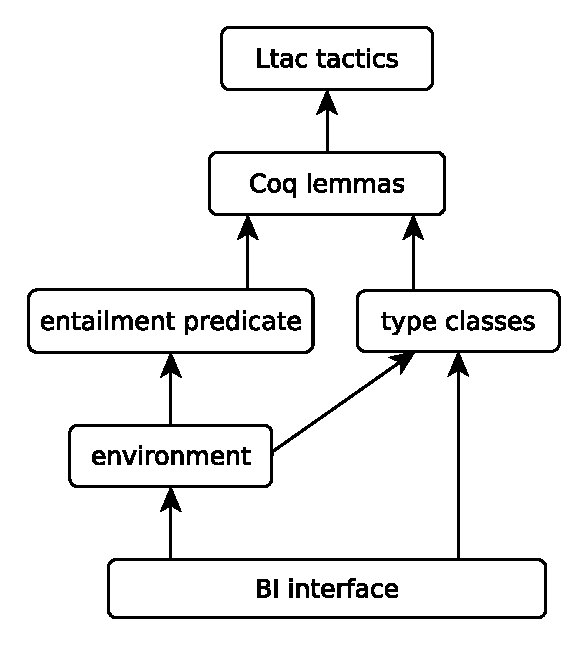
\includegraphics[width=0.5\linewidth]{ipm-diagram}
  \caption{structure of the implementation of IPM}
  \label{fig:ipm-diagram}
\end{figure}


\begin{itemize}
\item The base layer of the implementation is a BI interface, which user instantiates with their logic and can profit from the existing infrastructure.
\item On top of the BI interface MoSeL defines environments and entailment predicates. These are used to make proofs of ``Coq tactics'' easier and typeclasses allow for more general unification and proof search.
\item ``Coq tactics'' themselves are verified transformations of the goal, the simplest instance being \coqe{tac_ex_falso}, which looks as follows:\\
\coqe{Lemma tac_ex_falso Delta Q : envs_entails Delta False → envs_entails Delta Q.}.
\item These transformations are then applied by Ltac1 (or Ltac2, in the reimplementation) programs, which can combine them, use specialized tactics for the subgoals they generate and handle errors.
  This is described in section~\ref{sec:ltac2-tactics-mosel}.
\end{itemize}

\subsubsection{BI interface}
\label{subsubsec:bi-interface}

There are five main components, starting with a base interface for BI logic, which we mentioned before and which \citet{krebbersMoSeLGeneralExtensible2018} call MoBI interfaces, for Modal BI.

We include it here, with some omissions:
\begin{coq}
Structure bi := Bi {
  bi_car :> Type;
  bi_dist : Dist bi_car;
  bi_emp : bi_car;
  bi_and : bi_car → bi_car → bi_car;
  bi_forall : forall A, (A → bi_car) → bi_car;
  bi_sep : bi_car → bi_car → bi_car;
  bi_wand : bi_car → bi_car → bi_car;
  bi_persistently : bi_car → bi_car;
  bi_pure : Prop → bi_car;
  bi_bi_mixin : BiMixin $\ldots$;
  $\ldots$
}.
\end{coq}

Where \coqe{BiMixin} is a field that describes axioms that connectives should satisfy, from associativity of separating conjunction to elimination rule for persistent modality.
With some notation definitons this allows writing and proving BI propositions, only requiring an instance of \coqe{bi}.

\begin{minipage}{\linewidth}
\begin{coq}
Context {PROP : bi}.
Lemma persistently_mono P Q : (P |- Q) → <pers> P |- <pers> Q.
\end{coq}
\end{minipage}

Proving such statement, however, at this point still requires applying axioms from \coqe{bi} by hand.

\subsubsection{Environments and entailment predicate}
\label{subsubsec:environment-entailment-pred}

In order to define IPM entailment, we first define contexts.
In general, since most of the tactics only have to deal with one hypothesis from the context or don't even touch existing ones (like \coqe{iIntro}), \citet{krebbersMoSeLGeneralExtensible2018} use deep embedding to allow easier syntactical transformations.

Environments are defined as association lists with identifiers used as keys and BI propositions as values.

\begin{coq}
Inductive ident :=
  | IAnon : positive -> ident
  | INamed :> string -> ident
Inductive env (A : Type) : Type :=
  | Enil : env A
  | Esnoc : env A -> ident -> A -> env A.
\end{coq}

However, as described above MoSeL entailment predicate includes two context: spatial and intuitionistic, so we have to define another structure to include both:

\begin{figure}[H]
\centering
\begin{coq}
Record envs (PROP : bi) := Envs {
  env_intuitionistic : env PROP;
  env_spatial : env PROP;
  env_counter : positive (** A counter to generate fresh hypothesis names *)
}.
\end{coq}
\caption{Definition of MoSeL environment in Coq}
\label{fig:coq_envs}
\end{figure}


Then we can define entailment predicate, which includes not only both contexts, but also a proof that identifiers in each context are unique \coqe{envs_wf $\Delta \urcorner$}.
\begin{coq}
  Definition envs_entails {PROP} ($\Delta$ : envs PROP) (Q : PROP):
  $\ulcorner$ envs_wf $\Delta \urcorner$ /\ $\intuit$ [$\wedge$] env_intuitionistic $\Delta$ * [*] env_spatial $\Delta$ |- Q
\end{coq}

Here \coqe{[*]} is an iterated separating conjunction, defined on lists as folds with respective operation, the same way as it was defined in theoretical presentation.

At this point we can already make some statements in both readable and easy to prove form, such as \coqe{tac_ex_falso}, which we mentioned before.\\
\coqe{Lemma tac_ex_falso Delta Q : envs_entails Delta False → envs_entails Delta Q.}

\subsubsection{Typeclasses}
\label{subsubsec:typeclasses}

Typeclasses serve multiple purposes in MoSeL development, here we are going to describe only couple of simplest instances needed for \coqe{iAssumption}.
The primary idea is to automatize simple parts of proof search via logic programming.

The first example we are going to look at are \coqe{Affine} and \coqe{AffineEnv}.
The former is defined simply as
\begin{coq}
Class Affine {PROP : bi} (Q : PROP) := affine : Q |- emp.
\end{coq}

With instances covering both basic connectives
\begin{coq}
Global Instance emp_affine : Affine emp.
Global Instance and_affine_l P Q : Affine P → Affine (P /\ Q).
Global Instance and_affine_r P Q : Affine Q → Affine (P /\ Q).
Global Instance sep_affine P Q : Affine P → Affine Q → Affine (P * Q).
$\ldots$
\end{coq}

And modalities
\begin{coq}
Global Instance affinely_affine P : Affine (<affine> P).
$\ldots$
\end{coq}

For the environment to be affine we simply require all resources in the context to be affine and declare instances for both constructors.
\begin{coq}
Class AffineEnv (Γ : env PROP) := affine_env : Forall Affine Γ.
Global Instance affine_env_nil : AffineEnv Enil.
Global Instance affine_env_snoc Γ i P :
  Affine P → AffineEnv Γ → AffineEnv (Esnoc Γ i P).
\end{coq}

The next example is slightly more involved and concerns entailment of one proposition with another.
To be more precise, we want to define a typeclass which corresponds to intuitive ``\(P\) is almost the same as \(Q\) and P entails Q''.
\begin{coq}
Class FromAssumption {PROP : bi} (p : bool) (P Q : PROP) :=
  from_assumption : $\intuit$?p P |- Q.
\end{coq}

There are two subclasses of it, providing instances where either the first or the second proposition is treated as an input.
\begin{coq}
Class KnownLFromAssumption {PROP : bi} (p : bool) (P Q : PROP) :=
  knownl_from_assumption :> FromAssumption p P Q.
Class KnownRFromAssumption {PROP : bi} (p : bool) (P Q : PROP) :=
  knownr_from_assumption :> FromAssumption p P Q.
\end{coq}

The difference between their instances is that for \coqe{KnownLFromAssumption} we ``match'' input \(P\) with structural rules and Q is an output and vice-versa for \coqe{KnownRFromAssumption}.
This allows for more effective search, but for our purposes it is a mere technicality, so we will only consider \coqe{KnownRFromAssumption}.

\begin{coq}
Lemma from_assumption_exact {PROP : bi} p (P : PROP) : FromAssumption p P P.
\end{coq}

While the simplest instance of this is just an identity \coqe{P |- P}, there are several more defined in MoSeL, which generalize it.
For example, given that we can prove \(\intuit P \vdash Q\), we can also prove \(\intuit P \vdash \affine Q\) and  \(\intuit P \vdash \intuit Q\).
\begin{coq}
Global Instance from_assumption_affinely_r P Q :
  FromAssumption true P Q → KnownRFromAssumption true P ($\affine$ Q).
Global Instance from_assumption_intuitionistically_r P Q :
  FromAssumption true P Q → KnownRFromAssumption true P ($\intuit$ Q).
\end{coq}

\subsubsection{Coq tactics}
\label{sec:coq-tactics}

As mentioned above, Coq tactics are verified goal transformations, which can be as simple as rules for \coqe{exfalso}, but also more advanced, like the one for \coqe{assumption}.

The idea is that we are provided an identifier of the resource that is in the context and should check all side conditions: the resource is indeed there, it coincides with the goal and other resources can be safely discarded.

\begin{figure}[H]
\begin{coq}
Lemma tac_assumption Delta i p P Q :
  envs_lookup i Delta = Some (p,P) →
  FromAssumption p P Q →
  (let Delta' := envs_delete true i p Delta in
   if env_spatial_is_nil Delta' then TCTrue
   else TCOr (Absorbing Q) (AffineEnv (env_spatial Delta'))) →
  envs_entails Delta Q.
\end{coq}
\caption{\coqe{tac_assumption} definition}
\label{fig:tac-assumption}
\end{figure}

\coqe{envs_lookup} returns a boolean for the context it found identifier \coqe{i} within and proposition \(P\) that was associated with it.

Second assumption guarantees that \(P\) entails \(Q\) and the last one checks that we can discard the rest of the spatial resrouces in \(\Delta\).
If spatial context is empty, there is nothing to discard, but otherwise either the whole environment must be affine, or the goal should be able to absorb them:
\(\Absorbing Q \defeq \forall Q, P * Q \vdash \absorb P\).

No other subgoals are generated, since this is a leaf of a derivation.

\section{Ltac2 tactics in MoSeL}
\label{sec:ltac2-tactics-mosel}

The final piece of the puzzle is Ltac2 layer.
While Coq tactics provide verified goal transformations, they require several inputs.
The balance between what should go into a Coq statement and Ltac2 function is about how easy is it to verify something.

Turning again to \coqe{iAssumption}, the idea is that a user doesn't provide explicit identifier of the resource they have in mind, instead tactic is supposed to find it on its own.

Simply asserting existence of such identifier in a Coq lemma doesn't solve anything, since ultimately we have to apply this transformation to the goal and user will have to provide it, hence universally quantified identifier in the definition of the Coq lemma~\ref{fig:tac-assumption}.
Instead, we go through all elements of the environment in Ltac2 and try to apply the lemma with each one.

\begin{figure}
\begin{coq}
Ltac2 i_assumption () :=
  let rec find (p : coq_bool) (g : ipm_env) (q : ipm_prop) :=
      lazy_match! g with
      | Esnoc ?gg ?j ?pp =>
        first [ refine '(tac_assumption _ \$j \$p \$pp _ _ _ _) >
                [ pm_reflexivity () (* for the lookup *)
                | i_solve_tc () (* perform typeclass search for FromAssumption*)
                | pm_reduce (); (* evaluate env_delete and if-branch *)
                  i_solve_tc ()]
              | find p gg q]
      end
  in
  lazy_match! goal with
  | [|- envs_entails (Envs ?gp ?gs _) ?q] =>
     first [ find '(true) gp q
           | find '(false) gs q
           | i_assumption_coq ()
           | Control.zero (Iriception (of_string "no assumption matching " ++
                                       of_constr q ++
                                       of_string " was found"))]
  end.
\end{coq}
\caption{\coqe{i_assumption} definition}
\label{fig:i-assumption-def}
\end{figure}

The listing is in figure~\ref{fig:i-assumption-def}.
Since there are two contexts to go through, we factor out recursion into \coqe{find} function, which takes a Boolean flag \coqe{p} to tell apart spatial and intuitionistic context, context \coqe{g} and proposition \coqe{q}.
Then we apply \coqe{tac_assumption} defined above~\ref{fig:tac-assumption} and discharge the goals with specialized tactics.
The first subgoal \coqe{envs_lookup i Delta = Some (p,P)} is computational, so \coqe{pm_reflexivity ()} performs evaluation and tries \coqe{reflexivity} tactic.
The other two concern type classes, so we use a wrapper around \coqe{typeclasses eauto} to solve them.

The only part which wasn't described so far is \coqe{i_assumption_coq ()}.
This is an example of tactics composition -- \coqe{i_assumption_coq} is applying a different lemma from \coqe{tac_assumption}, which tries to find an assumption of shape \(\vdash Q\) in the Coq context instead of IPM context.

This example also showcases some error handling in the last case, if none of the cases listed before it succeed.

\subsection{The examplary proof}
\label{sec:examplary-proof-in-ltac2-mosel}

We now show what the proof looks like in the reimplemented version of MoSeL.

The full listing is in figure~\ref{fig:example-proof-mosel-ltac2}.
Since we didn't touch environment or rendering of the goals, for the user only tactics changed and everything else stayed the same, including the proof states.

Perhaps, the biggest difference from the Ltac1 version is the lack of notations.
However, this is not Ltac2's fault, but rather ours -- we didn't focus on them and this aspect can still be improved.

\begin{figure}
\begin{coq}
Lemma example {A : Type} (P : PROP) (Phi Psi : A → PROP) :
  P * (exists a, (Phi a) \/ (Psi a)) -* exists a, (P * Phi a) \/ (P * Psi a).
Proof.
  i_intro_named "H".
  i_and_destruct '(INamed "H") '(INamed "HP") '(INamed "HE").
  i_exist_destruct '(INamed "HE") as x '(INamed "HE").
  i_or_destruct '(INamed "HE") '(INamed "H1") '(INamed "H2").
  - i_exists$\text{~}$x. i_left (). i_split_l ["HP"] ;; i_assumption ().
  - i_exists$\text{~}$x. i_right (). i_split_l ["HP"] ;; i_assumption ().
Qed.
\end{coq}
\caption{An example of a proof using Ltac2 version of MoSeL}
\label{fig:example-proof-mosel-ltac2}
\end{figure}


\subsection{Potential and observed improvements from translation to Ltac2}
\label{sec:impr-from-transl}

While translating implementation from Ltac1 to Ltac2, we encountered several points where Ltac2 was particularly useful.

\paragraph{Fix arities from original IPM}

In the original implementation there aren't tactics of arbitrary arity.
Instead, due to Ltac limitations, developers were forced to define several variants of tactics, each with fixed arity.

\begin{coq}
Tactic Notation "iExists" uconstr(x1) "," uconstr(x2) :=
  iExists x1; iExists x2.
Tactic Notation "iExists" uconstr(x1) "," uconstr(x2) "," uconstr(x3) :=
  iExists x1; iExists x2, x3.
$\ldots$
\end{coq}

With Ltac2 we can use scopes for lists, which allow arbitrary arities.
The example above would look as follows:

\begin{coq}
  Ltac2 Notation "iExists" lc(list1(thunk(seq(constr, with_bindings)), ",")) :=
  i_exists$\text{~}$lc.
\end{coq}

Where \coqe{i_exists} iterates over the list and applies \coqe{iExists} to each element.

\paragraph{Error messages}

Another pain point of Ltac development is lack of proper error handling.

With Ltac2 there two features that help -- we can define our own custom error classes and there is a proper error handling mechanism, which allows us to match on the error thrown.

As with the \coqe{i_assumption} above, there are multiple instances of nesting tactics within each other.
One way to improve error message thrown by iAssumption would be to catch potential error thrown by \coqe{i_assumption_coq} and append it to the error message produced in \coqe{i_assumption}, so that user can see why the tactic failed.

\section{Desirable features in Ltac2}

However, there also were several features that we wished Ltac2 had and that impacted the scope of potential improvements.

\paragraph{User-defined scopes}

Perhaps, one of the useful features of the original IPM implementation that is missing from our implementation is intropatterns.
The proper way to define them with Ltac2 would be to extend datatype for intropattern with IPM-specific symbols and then parse it with a custom scope.

Unfortunately, the latter isn't currently possible without extending OCaml implementation of Ltac2, either via forking Coq or using an Ocaml plugin that modifies Ltac2 grammar.

\paragraph{User-defined pretty-printing}
Another missing feature would be lack of user-defined printing rules.
At the moment this mostly impacts error printing, since we have to rely on the Ltac2 pretty-printer, as notations are parsing-only.

\paragraph{notypeclasses refine}

Ltac2 also currently lacks a variant of \coqe{refine}, which doesn't resolve typeclasses on the application.
This tactic is heavily used in MoSeL development.

\paragraph{Interoperability between Ltac1 and Ltac2}

While the goal of the rewriting was to give platform for further experiments, some of the tactics were easier to import.
And while there is a way to call Ltac1 tactics from Ltac2 code, there is no proper way to pass return values there or back.
I.e.\ \href{https://gitlab.mpi-sws.org/iris/string-ident/}{iris string-ident} has to pass terms through the goal to get the result from one to another.

%%% Local Variables:
%%% mode: latex
%%% TeX-master: "thesis"
%%% TeX-parse-self: t
%%% TeX-auto-save: t
%%% reftex-cite-format: natbib
%%% reftex-default-bibliography: ("/home/buzzer/my-dir/ed/uni/saar/prjcts/iris/npm/tex/TacticsProofs.bib")
%%% End: